\documentclass{standalone}
\usepackage{tikz}
\usetikzlibrary{patterns, positioning}
\usepackage[sfdefault]{ClearSans} %% option 'sfdefault' activates Clear Sans as the default text font
\usepackage[T1]{fontenc}

\begin{document}
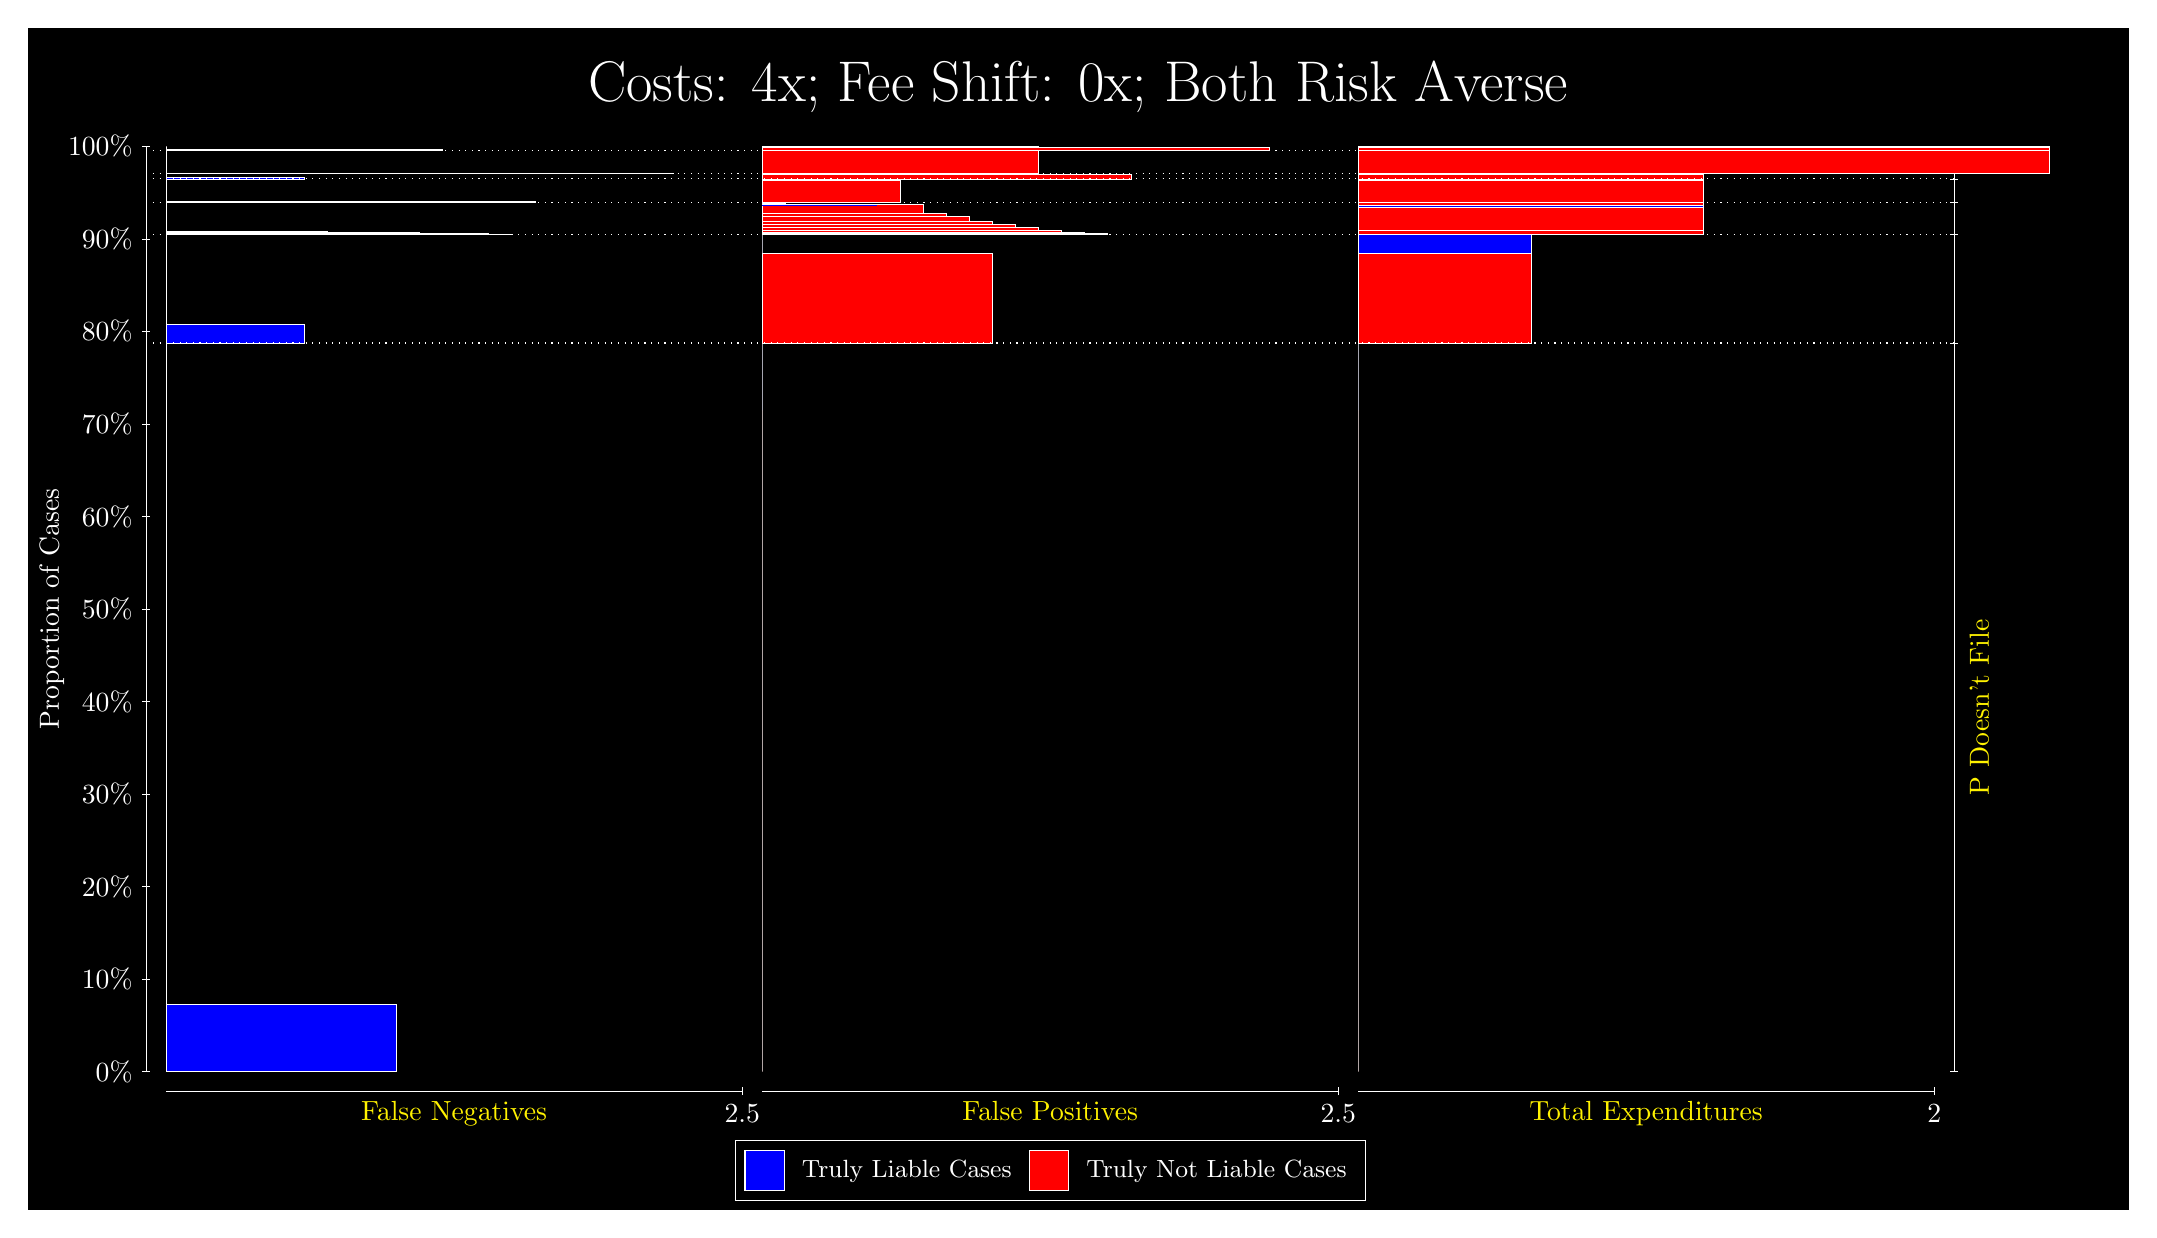
\begin{tikzpicture}
\draw[fill=black] (0,0) rectangle (26.667,15);
\draw[text=white] (0,13.5) rectangle (26.667,15) node[midway] {\huge Costs: 4x; Fee Shift: 0x; Both Risk Averse};
\draw[white, very thin] (1.5,1.75) -- (1.5,13.5);
\node[rotate=90, text=white, anchor=center] at (0.3, 7.625) {Proportion of Cases};
\draw[white, very thin] (1.45,1.75) -- (1.55,1.75);
\node[text=white, anchor=east] at (1.45, 1.75) {0\%};
\draw[white, very thin] (1.45,2.925) -- (1.55,2.925);
\node[text=white, anchor=east] at (1.45, 2.925) {10\%};
\draw[white, very thin] (1.45,4.1) -- (1.55,4.1);
\node[text=white, anchor=east] at (1.45, 4.1) {20\%};
\draw[white, very thin] (1.45,5.275) -- (1.55,5.275);
\node[text=white, anchor=east] at (1.45, 5.275) {30\%};
\draw[white, very thin] (1.45,6.45) -- (1.55,6.45);
\node[text=white, anchor=east] at (1.45, 6.45) {40\%};
\draw[white, very thin] (1.45,7.625) -- (1.55,7.625);
\node[text=white, anchor=east] at (1.45, 7.625) {50\%};
\draw[white, very thin] (1.45,8.8) -- (1.55,8.8);
\node[text=white, anchor=east] at (1.45, 8.8) {60\%};
\draw[white, very thin] (1.45,9.975) -- (1.55,9.975);
\node[text=white, anchor=east] at (1.45, 9.975) {70\%};
\draw[white, very thin] (1.45,11.15) -- (1.55,11.15);
\node[text=white, anchor=east] at (1.45, 11.15) {80\%};
\draw[white, very thin] (1.45,12.325) -- (1.55,12.325);
\node[text=white, anchor=east] at (1.45, 12.325) {90\%};
\draw[white, very thin] (1.45,13.5) -- (1.55,13.5);
\node[text=white, anchor=east] at (1.45, 13.5) {100\%};

\draw[white, very thin] (24.457,1.75) -- (24.457,13.5);
\draw[white, very thin] (24.407,1.75) -- (24.507,1.75);
\node[anchor=west] at (24.407, 1.75) {};
\draw[white, very thin] (24.407,11.002) -- (24.507,11.002);
\node[anchor=west] at (24.407, 11.002) {};
\draw[white, very thin] (24.407,12.383) -- (24.507,12.383);
\node[anchor=west] at (24.407, 12.383) {};
\draw[white, very thin] (24.407,12.792) -- (24.507,12.792);
\node[anchor=west] at (24.407, 12.792) {};
\draw[white, very thin] (24.407,13.086) -- (24.507,13.086);
\node[anchor=west] at (24.407, 13.086) {};
\draw[white, very thin] (24.407,13.158) -- (24.507,13.158);
\node[anchor=west] at (24.407, 13.158) {};
\draw[white, very thin] (24.407,13.45) -- (24.507,13.45);
\node[anchor=west] at (24.407, 13.45) {};
\draw[white, very thin] (24.407,13.5) -- (24.507,13.5);
\node[anchor=west] at (24.407, 13.5) {};

\draw[white, very thin, fill=blue] (1.75,1.75) rectangle (4.6775,2.6022);
\draw[white, very thin, fill=red] (1.75,2.6022) rectangle (1.75,11.002);
\draw[white, very thin, fill=blue] (1.75,11.002) rectangle (3.5065,11.245);
\draw[white, very thin, fill=red] (1.75,11.245) rectangle (1.75,12.383);
\draw[white, very thin, fill=blue] (1.75,12.383) rectangle (6.1413,12.388);
\draw[white, very thin, fill=blue] (1.75,12.388) rectangle (5.8486,12.391);
\draw[white, very thin, fill=blue] (1.75,12.391) rectangle (5.5558,12.398);
\draw[white, very thin, fill=blue] (1.75,12.398) rectangle (5.2631,12.402);
\draw[white, very thin, fill=blue] (1.75,12.402) rectangle (4.9703,12.407);
\draw[white, very thin, fill=blue] (1.75,12.407) rectangle (4.6775,12.41);
\draw[white, very thin, fill=blue] (1.75,12.41) rectangle (4.3848,12.413);
\draw[white, very thin, fill=blue] (1.75,12.413) rectangle (4.092,12.414);
\draw[white, very thin, fill=blue] (1.75,12.414) rectangle (3.7993,12.415);
\draw[white, very thin, fill=red] (1.75,12.415) rectangle (1.75,12.792);
\draw[white, very thin, fill=blue] (1.75,12.792) rectangle (6.4341,12.807);
\draw[white, very thin, fill=red] (1.75,12.807) rectangle (1.75,13.086);
\draw[white, very thin, fill=blue] (1.75,13.086) rectangle (3.5065,13.105);
\draw[white, very thin, fill=red] (1.75,13.105) rectangle (1.75,13.158);
\draw[white, very thin, fill=blue] (1.75,13.158) rectangle (8.1906,13.163);
\draw[white, very thin, fill=red] (1.75,13.163) rectangle (1.75,13.45);
\draw[white, very thin, fill=blue] (1.75,13.45) rectangle (5.2631,13.457);
\draw[white, very thin, fill=red] (1.75,13.457) rectangle (1.75,13.5);
\draw[white, very thin, fill=red] (9.3189,1.75) rectangle (9.3189,10.149);
\draw[white, very thin, fill=blue] (9.3189,10.149) rectangle (9.3189,11.002);
\draw[white, very thin, fill=red] (9.3189,11.002) rectangle (12.246,12.139);
\draw[white, very thin, fill=blue] (9.3189,12.139) rectangle (9.3189,12.383);
\draw[white, very thin, fill=red] (9.3189,12.383) rectangle (13.71,12.396);
\draw[white, very thin, fill=red] (9.3189,12.396) rectangle (13.417,12.408);
\draw[white, very thin, fill=red] (9.3189,12.408) rectangle (13.125,12.435);
\draw[white, very thin, fill=red] (9.3189,12.435) rectangle (12.832,12.468);
\draw[white, very thin, fill=red] (9.3189,12.468) rectangle (12.539,12.513);
\draw[white, very thin, fill=red] (9.3189,12.513) rectangle (12.246,12.545);
\draw[white, very thin, fill=red] (9.3189,12.545) rectangle (11.954,12.612);
\draw[white, very thin, fill=red] (9.3189,12.612) rectangle (11.661,12.648);
\draw[white, very thin, fill=red] (9.3189,12.648) rectangle (11.368,12.76);
\draw[white, very thin, fill=blue] (9.3189,12.76) rectangle (10.783,12.761);
\draw[white, very thin, fill=blue] (9.3189,12.761) rectangle (10.49,12.762);
\draw[white, very thin, fill=blue] (9.3189,12.762) rectangle (10.197,12.765);
\draw[white, very thin, fill=blue] (9.3189,12.765) rectangle (9.9044,12.768);
\draw[white, very thin, fill=blue] (9.3189,12.768) rectangle (9.6116,12.773);
\draw[white, very thin, fill=blue] (9.3189,12.773) rectangle (9.3189,12.792);
\draw[white, very thin, fill=red] (9.3189,12.792) rectangle (11.075,13.071);
\draw[white, very thin, fill=blue] (9.3189,13.071) rectangle (9.3189,13.086);
\draw[white, very thin, fill=red] (9.3189,13.086) rectangle (14.003,13.139);
\draw[white, very thin, fill=blue] (9.3189,13.139) rectangle (11.075,13.158);
\draw[white, very thin, fill=red] (9.3189,13.158) rectangle (12.832,13.445);
\draw[white, very thin, fill=blue] (9.3189,13.445) rectangle (9.9044,13.45);
\draw[white, very thin, fill=red] (9.3189,13.45) rectangle (15.759,13.493);
\draw[white, very thin, fill=blue] (9.3189,13.493) rectangle (12.832,13.5);
\draw[white, very thin, fill=red] (16.888,1.75) rectangle (16.888,10.149);
\draw[white, very thin, fill=blue] (16.888,10.149) rectangle (16.888,11.002);
\draw[white, very thin, fill=red] (16.888,11.002) rectangle (19.083,12.139);
\draw[white, very thin, fill=blue] (16.888,12.139) rectangle (19.083,12.383);
\draw[white, very thin, fill=red] (16.888,12.383) rectangle (21.279,12.428);
\draw[white, very thin, fill=blue] (16.888,12.428) rectangle (21.279,12.433);
\draw[white, very thin, fill=red] (16.888,12.433) rectangle (21.279,12.725);
\draw[white, very thin, fill=blue] (16.888,12.725) rectangle (21.279,12.749);
\draw[white, very thin, fill=red] (16.888,12.749) rectangle (21.279,12.788);
\draw[white, very thin, fill=blue] (16.888,12.788) rectangle (21.279,12.792);
\draw[white, very thin, fill=red] (16.888,12.792) rectangle (21.279,13.071);
\draw[white, very thin, fill=blue] (16.888,13.071) rectangle (21.279,13.086);
\draw[white, very thin, fill=red] (16.888,13.086) rectangle (21.279,13.139);
\draw[white, very thin, fill=blue] (16.888,13.139) rectangle (21.279,13.158);
\draw[white, very thin, fill=red] (16.888,13.158) rectangle (25.67,13.445);
\draw[white, very thin, fill=blue] (16.888,13.445) rectangle (25.67,13.45);
\draw[white, very thin, fill=red] (16.888,13.45) rectangle (25.67,13.493);
\draw[white, very thin, fill=blue] (16.888,13.493) rectangle (25.67,13.5);
\draw[white, dotted] (1.5,11.002) -- (24.457,11.002);
\draw[white, dotted] (1.5,12.383) -- (24.457,12.383);
\draw[white, dotted] (1.5,12.792) -- (24.457,12.792);
\draw[white, dotted] (1.5,13.086) -- (24.457,13.086);
\draw[white, dotted] (1.5,13.158) -- (24.457,13.158);
\draw[white, dotted] (1.5,13.45) -- (24.457,13.45);
\draw[white, very thin] (1.75,1.5) -- (9.0689,1.5);
\node[text=yellow, anchor=north] at (5.4094, 1.5) {False Negatives};
\draw[white, very thin] (9.0689,1.45) -- (9.0689,1.55);
\node[text=white, anchor=north] at (9.0689, 1.45) {2.5};

\draw[white, very thin] (9.3189,1.5) -- (16.638,1.5);
\node[text=yellow, anchor=north] at (12.978, 1.5) {False Positives};
\draw[white, very thin] (16.638,1.45) -- (16.638,1.55);
\node[text=white, anchor=north] at (16.638, 1.45) {2.5};

\draw[white, very thin] (16.888,1.5) -- (24.207,1.5);
\node[text=yellow, anchor=north] at (20.547, 1.5) {Total Expenditures};
\draw[white, very thin] (24.207,1.45) -- (24.207,1.55);
\node[text=white, anchor=north] at (24.207, 1.45) {2};

\node[text=yellow, centered, rotate=90] at (24.777, 6.3758) {P Doesn't File};







\draw (12.978300999999998,1.5) node[draw=none] (baseCoordinate) {};
\begin{scope}[align=center]
        \matrix[scale=0.5, draw=white, below=0.5cm of baseCoordinate, nodes={draw}, column sep=0.1cm]{
            \node[rectangle, draw, minimum width=0.5cm, minimum height=0.5cm, fill=blue] {}; &
            \node[draw=none, font=\small, text=white] (B) {Truly Liable Cases}; &
            \node[rectangle, draw, minimum width=0.5cm, minimum height=0.5cm, fill=red] {}; &
            \node[draw=none, font=\small, text=white] (B) {Truly Not Liable Cases}; \\
            };
\end{scope}

\end{tikzpicture}
\end{document}